\ifx\wholebook\relax \else

\documentclass[b5paper]{article}
\usepackage[nomarginpar
  %, margin=.5in
]{geometry}

\addtolength{\oddsidemargin}{-0.05in}
\addtolength{\evensidemargin}{-0.05in}
\addtolength{\textwidth}{0.1in}

\usepackage[en]{../../prelude}

\setcounter{page}{1}

\begin{document}

\title{Insertion sort}

\author{Xinyu LIU
\thanks{{\bfseries Xinyu LIU} \newline
  Email: liuxinyu99@hotmail.com \newline}
  }

\maketitle
\fi

\markboth{Insertion sort}{Elementary Algorithms}

\ifx\wholebook\relax
\chapter{Insertion sort}
\numberwithin{Exercise}{chapter}
\fi

\section{Introduction}
\label{sec:isort-introduction} \index{insertion sort}

\lstset{frame = single}
Insertion sort is a straightforward sort algorithm\footnote{We skip the `Bubble sort' method}. We give its preliminary definition for list in chapter 1. For a collection of comparable elements, we repeatedly pick one, insert them to a list and maintain the ordering. As every insertion takes linear time, its performance is bound to $O(n^2)$ where $n$ is the number of elements. This performance is not as good as the divide and conqueror sort algorithms, like quick sort and merge sort. However, we can still find its application today. For example, a well tuned quick sort implementation falls back to insertion sort for small data set. The idea of insertion sort is similar to sort a deck of a poker cards(\cite{CLRS} pp.15). The cards are shuffled. A player takes card one by one. At any time, all cards on hand are sorted. When draws a new card, the player inserts it in proper position according to the order of points as shown in \cref{fig:hand-of-cards}.

\begin{figure}[htbp]
  \centering
  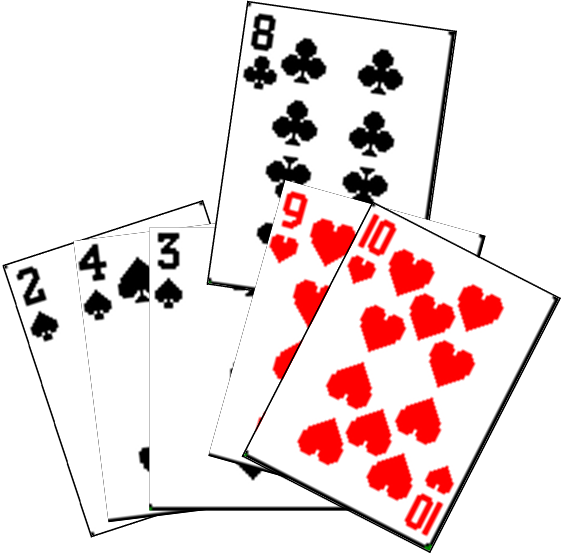
\includegraphics[scale=0.5]{img/card-deck}
  \caption{Insert card 8 to a deck.}
  \label{fig:hand-of-cards}
\end{figure}

Based on this idea, we can implement insertion sort as below:

\begin{algorithmic}[1]
\Function{Sort}{$A$}
  \State $S \gets [\ ]$
  \For{each $a \in A$}
    \State \Call{Insert}{$a, S$}
  \EndFor
  \State \Return $S$
\EndFunction
\end{algorithmic}

We store the sorted result in a new array, alternatively, we can change it to in-place:

\begin{algorithmic}[1]
\Function{Sort}{$A$}
  \For{$i \gets 2$ to $|A|$}
    \State ordered insert $A[i]$ to $A[1...(i-1)]$
  \EndFor
\EndFunction
\end{algorithmic}

Where the index $i$ ranges from 1 to $n = |A|$. We start from 2, because the singleton sub-array of $A[1]$ is ordered. When process the $i$-th element, all elements before $i$ are sorted. We continuously insert elements till $n$, as shown in \cref{fig:in-place-sort}.

\begin{figure}[htbp]
  \centering
  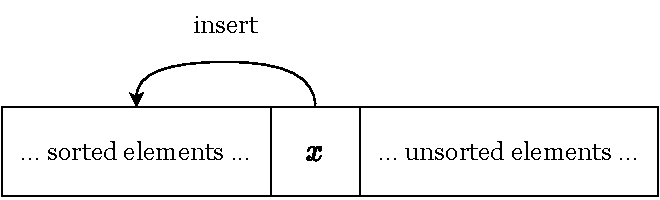
\includegraphics[scale=0.7]{img/insert-sort}
  \caption{Continuously insert elements to the sorted part.}
  \label{fig:in-place-sort}
\end{figure}

\section{Insertion}
\index{insertion sort!insertion}

In chapter 1, we define the ordered insertion for list. For array, we scan to locate the insert position either from left or right. Below algorithm is from right:

\begin{algorithmic}[1]
\Function{Sort}{$A$}
  \For{$i \gets 2$ to $|A|$}
    \Comment{Insert $A[i]$ to $A[1...(i-1)]$}
    \State $x \gets A[i]$ \Comment{Save $A[i]$ to $x$}
    \State $j \gets i-1$
    \While{$j > 0$ and $x < A[j]$ }
      \State $A[j+1] \gets A[j]$
      \State $j \gets j - 1$
    \EndWhile
    \State $A[j+1] \gets x$
  \EndFor
\EndFunction
\end{algorithmic}

It's expensive to insert at arbitrary position, as array stores elements continuously. When insert $x$ at position $i$, we need shift all elements after $i$ (i.e. $A[i + 1], A[i + 2], ...$) right. then put $x$ in the freed cell, as shown in \cref{fig:array-shift}.

\begin{figure}[htbp]
  \centering
  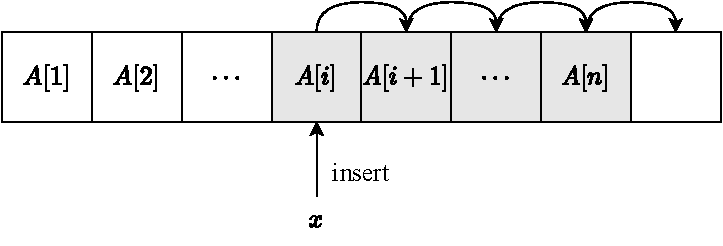
\includegraphics[scale=0.7]{img/array-shift}
  \caption{Insert $x$ to $A$ at $i$.}
  \label{fig:array-shift}
\end{figure}

For the array of length $n$, suppose after comparing $x$ to the first $i$ elements, we located the position to insert. Then we shift the rest $n - i + 1$ elements, and put $x$ in the $i$-th cell. Overall, we traverse the entire array if scan from left. While, if scan from right, we examine $n - i + 1$ elements, and do the same amount of shifts. The insertion takes linear time no matter scans from left or right, hence the sort algorithm is bound to $O(n^2)$. We can also define a separated \textproc{Insert}() function, and call it inside the loop.

\begin{Exercise}\label{ex:isort-insert}
\Question{Implement the insert to scan from left to right.}
\Question{Define the insert function, and call it from the sort algorithm.}
\end{Exercise}

\begin{Answer}[ref = {ex:isort-insert}]
\Question{Implement the insert to scan from left to right.
\begin{Bourbaki}
Void insert([T] xs, T x) {
    Int i = 0, n = length(xs)
    append(xs, x)
    while i < n and xs[i] < x { i++ }
    while i < n {
        xs[n] = xs[n - 1]
        n = n - 1
    }
    xs[i] = x
}
\end{Bourbaki}
}
\Question{Define the insert function, and call it from the sort algorithm.
\begin{Bourbaki}
Void insert([T] xs, T x) {
    append(xs, x)
    Int i = length(xs) - 1
    while i > 0 and xs[i] < xs[i-1] {
        swap(xs[i], xs[i-1])
        i--
    }
}

[T] sort([T] xs) {
    [T] ys = []
    for x in xs {
        insert(ys, x)
    }
    return ys
}
\end{Bourbaki}
}
\end{Answer}

\section{Binary search}
\index{Insertion sort!binary search}

When insert a poker card, human does not scan, but takes a quick glance at the deck to locate the position. We can do this because the deck is sorted. Binary search is such a method that applies to ordered sequence.

\begin{algorithmic}[1]
\Function{Sort}{$A$}
  \For{$i \gets 2$ to $|A|$}
    \State $x \gets A[i]$
    \State $p \gets $ \Call{Binary-Search}{$x, A[1...(i-1)]$}
    \For{$j \gets i$ down to $p$}
      \State $A[j] \gets A[j-1]$
    \EndFor
    \State $A[p] \gets x$
  \EndFor
\EndFunction
\end{algorithmic}

Because the slice $A[1...(i-1)]$ is already ordered, to find the position $j$ such that$A[j-1] \leq x \leq A[j]$, we compare $x$ to the middle element $A[m]$, where $m = \lfloor \dfrac{i}{2} \rfloor$. If $x < A[m]$, we then recursively apply binary search to the first half; otherwise, we search the second half. As we halve the elements every time, binary search takes $O(\lg i)$ time to locate the insert position.

\begin{algorithmic}[1]
\Function{Binary-Search}{$x, A$}
  \State $l \gets 1, u \gets 1+|A|$
  \While{$l < u$}
    \State $m \gets \lfloor \dfrac{l+u}{2} \rfloor$
    \If{$A[m] = x$}
      \State \Return $m$ \Comment{Duplicated element}
    \ElsIf{$A[m] < x$}
      \State $l \gets m+1$
    \Else
      \State $u \gets m$
    \EndIf
  \EndWhile
  \State \Return $l$
\EndFunction
\end{algorithmic}

The improved sort algorithm is still bound to $O(n^2)$. The one with scan takes $O(n^2)$ comparisons and $O(n^2)$ shifts; with binary search, it takes $O(n \lg n)$ comparisons and $O(n^2)$ shifts.

%% \begin{Exercise}
%% \Question{Implement the recursive binary search.}
%% \end{Exercise}

\section{List}
\index{Insertion sort!linked-list setting}

With binary search, the total number of comparisons reduced to $O(n \lg n)$. However, as we need shift array cells when insert, the overall time is still bound to $O(n^2)$. On the other hand, when use list, the insert operation is constant time at a given node reference. In chapter 1, we define the insertion sort algorithm for list as below:

\be
\begin{array}{rcl}
sort\ [\ ] & = & [\ ] \\
sort\ (x \cons xs) & = & insert\ x\ (sort\ xs) \\
\end{array}
\ee

Or define with $foldr$ in Curried form: $sort = foldr\ insert\ [\ ]$. However, the list $insert$ algorithm still takes linear time, because we need scan to locate the insert position:

\be
\begin{array}{rcl}
insert\ x\ [\ ] & = & [x] \\
insert\ x\ (y \cons ys) & = & \begin{cases}
  x \leq y : & x : y : ys \\
  \text{otherwise}: & y : insert\ x\ ys \\
  \end{cases}
\end{array}
\ee

\label{sec:list-index-array}
Instead of using node reference, we can also realize list through an additional index array. For every element $A[i]$, $Next[i]$ stores the index to the next element follows $A[i]$, i.e. $A[Next[i]]$ is the next element of $A[i]$. There are two special indexes: for the tail node $A[m]$, we define $Next[m] = -1$, indicating it points to NIL; we also define $Next[0]$ to index the head element. With the index array, we can implement the insertion algorithm as below:

\begin{algorithmic}[1]
\Function{Insert}{$A, Next, i$}
  \State $j \gets 0$ \Comment{$Next[0]$ for head}
  \While{$Next[j] \neq -1$ and $A[Next[j]] < A[i]$}
    \State $j \gets Next[j]$
  \EndWhile
  \State $Next[i] \gets Next[j]$
  \State $Next[j] \gets i$
\EndFunction
\Statex
\Function{Sort}{$A$}
  \State $n \gets |A|$
  \State $Next = [1, 2, ..., n, -1]$ \Comment{$n + 1$ indexes}
  \For{$i \gets 1$ to $n$}
    \State \Call{Insert}{$A, Next, i$}
  \EndFor
  \State \Return $Next$
\EndFunction
\end{algorithmic}

With list, although the insert operation changes to constant time, we need traverse the list to locate the position. It is still bound to $O(n^2)$ times comparison. Unlike array, list does not support random access, hence we can not use binary search to speed up.

\begin{Exercise}\label{ex:list-index-array-reorder}
\Question{For the index array based list, we return the re-arranged index as result. Design an algorithm to re-order the original array $A$ from the index $Next$.}
\end{Exercise}

\begin{Answer}[ref = {ex:list-index-array-reorder}]
\Question{For the index array based list, we return the re-arranged index as result. Design an algorithm to re-order the original array $A$ from the index $Next$.
\begin{Bourbaki}
[K] reorder([K] xs, [Int] next) {
    Int i = -1
    [Int] ys = []
    while next[i] != -1 {
        append(ys, xs[next[i]])
        i = next[i]
    }
    return ys
}
\end{Bourbaki}
}
\end{Answer}

\section{Binary search tree}
\index{Insertion sort!binary search tree}

We drive into a corner. We want to improve both comparison and insertion at the same time, or will end up with $O(n^2)$ performance. For comparison, we need binary search to achieve $O(\lg n)$ time; on the other hand, we need change the data structure, because array can not support constant time insertion at a position. We introduce a powerful data structure in chapter 2, the binary search tree. It supports binary search from its definition by nature. At the same time, we can insert a new node in binary search tree fast at the given location.

\begin{algorithmic}[1]
\Function{Sort}{$A$}
  \State $T \gets \nil$
  \For{each $x \in A$}
    \State $T \gets $ \Call{Insert-Tree}{$T, x$}
  \EndFor
  \State \Return \Call{To-List}{$T$}
\EndFunction
\end{algorithmic}

Or $sort = toList \circ \textit{fromList}$ for list, where \textproc{Insert-Tree}(), \textproc{To-List}(), and \textit{fromList} are defined in chapter 2. In average case, the performance of tree sort is bound to $O(n \lg n)$. This is the lower limit of comparison based sort(\cite{Knuth-V3} pp.180-193). However, in the worst case that the tree is poor balanced the performance drops to $O(n^2)$.

Insertion sort is often used as the first example of sorting. It is straightforward and easy to implement. However its performance is quadratic. Insertion sort does not only appear in textbooks, it has practical use case in the quick sort implementation. It is an engineering practice to fallback to insertion sort when the number of elements is small.

\ifx\wholebook\relax \else
\section{Answers}
\shipoutAnswer

\begin{thebibliography}{99}

\bibitem{CLRS}
Thomas H. Cormen, Charles E. Leiserson, Ronald L. Rivest and Clifford Stein.
``Introduction to Algorithms, Second Edition''. ISBN:0262032937. The MIT Press. 2001

\bibitem{Knuth}
Donald E. Knuth. ``The Art of Computer Programming, Volume 3: Sorting and Searching (2nd Edition)''. Addison-Wesley Professional; 2 edition (May 4, 1998) ISBN-10: 0201896850 ISBN-13: 978-0201896855

\end{thebibliography}

\end{document}
\fi
